\documentclass{article}
\usepackage[utf8]{inputenc}
\usepackage{amsmath}
\usepackage{amssymb}
\usepackage{color}
\usepackage{graphicx}
\usepackage{float}
\usepackage{physics}
\title{report v0.tex }
\author{Henrik Linder}
\date{\today}
\begin{document}
\maketitle

Given the rates of protein production and decay as 
\begin{equation}
	k_p^{mRNA} = \frac{1}{600}[s^{-1}],\quad k_d = \frac{1}{1800}N_p[s^{-1}],
\end{equation}
we can describe the change in number of proteins $N_p$ as a function of time with the ODE 
\begin{equation}
	\label{eq:protein_ODE}
	\dv {N_p}{t} = k_p^{mRNA}  - k_dN_p .
\end{equation}
By setting $\dv {N_p}{t} = 0 $, we can see that we get a steady state solution when $k_p^{mRNA} = k_dN_p$, or 
\begin{equation}
	\label{eq:steady_state}
	N_p = 3.
\end{equation}


\begin{figure}[H]
	\centering
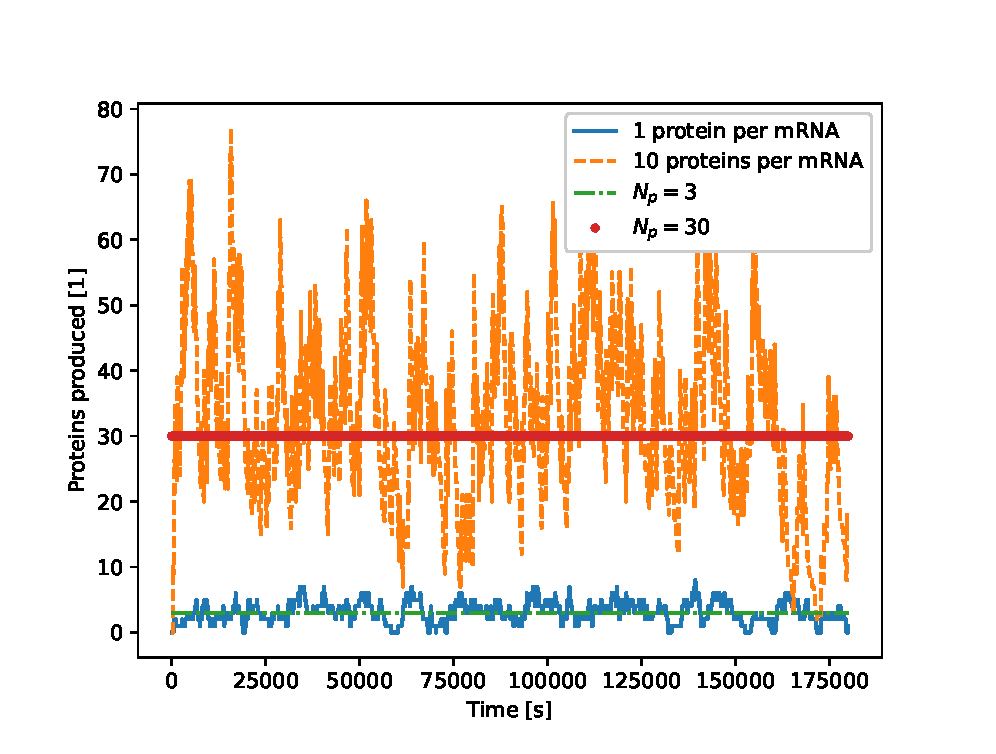
\includegraphics[width = \linewidth]{figs/task1_results_v3.eps}
	\label{fig:task1_results}
\end{figure}

\begin{figure}[H]
	\centering
	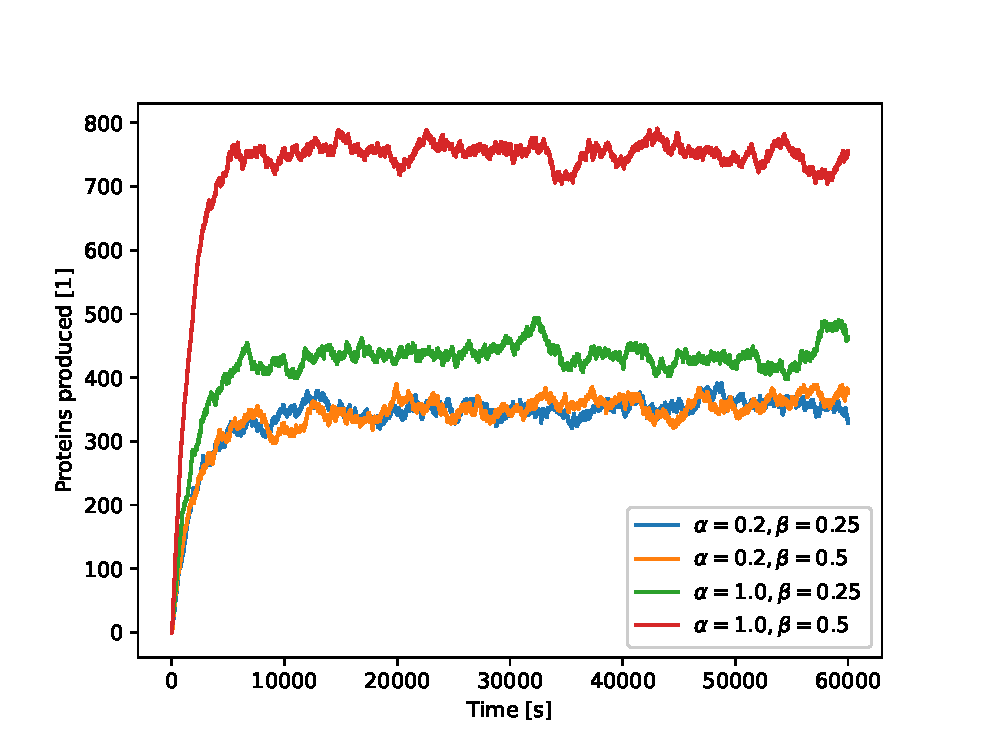
\includegraphics[width = \linewidth]{figs/task2_prot_prod_v4.eps}
	\label{fig:task2_prot_prod}
\end{figure}

\begin{figure}[H]
	\centering
	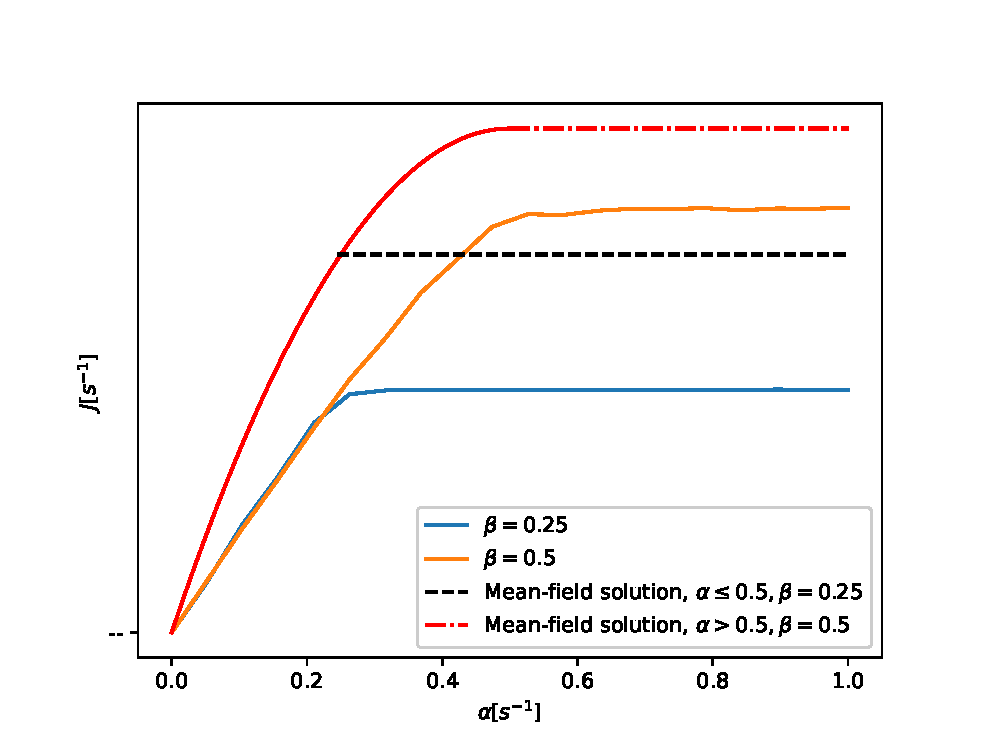
\includegraphics[width = \linewidth]{figs/task2_meanfield_v4.eps}
	\label{fig:task2_mean-field}
\end{figure}



\section{task3}
fano1 : 1.1537323139033988,  1.0293234725437235, 1.1255733414025437,  0.9870385180083185


fano cont. : 3.4324503269801925, 2.629365078890865, 2.212654090046395, 2.816569373857693




\end{document}
